%(BEGIN_QUESTION)
% Copyright 2006, Tony R. Kuphaldt, released under the Creative Commons Attribution License (v 1.0)
% This means you may do almost anything with this work of mine, so long as you give me proper credit

Tegn skjematiske diagrammer for følgende RTD-er:

$$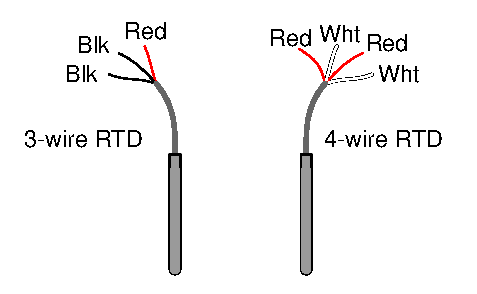
\includegraphics[width=15.5cm]{i00404x01.eps}$$

Vis deretter hvordan hver RTD-type kobles til inngangsterminalene på en RTD-temperaturtransmitter. Merk at hver transmitter kan konfigureres for ulike RTD-typer, vist symbolsk på fronten:

$$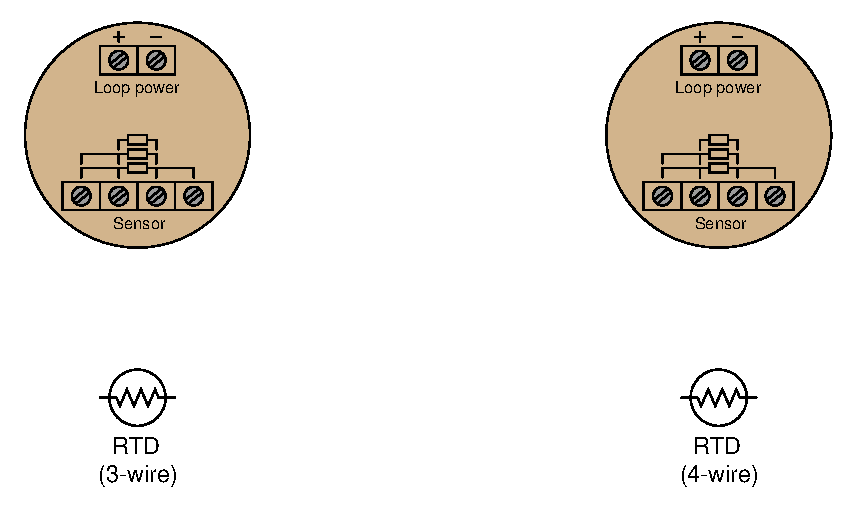
\includegraphics[width=15.5cm]{i00404x02.eps}$$

\vskip 20pt \vbox{\hrule \hbox{\strut \vrule{} {\bf Forslag til sokratisk diskusjon} \vrule} \hrule}

\begin{itemize}
\item{} Hva representerer vanlige farger for RTD-lederne?
\item{} Hvilken fordel har 4-leder RTD over 3-leder RTD som forsvarer ekstra kostnad og ekstra leder?
\item{} Tolk betydningen av boksformede motstandssymboler på transmitterfrontene. Viser disse hva som skal kobles til terminalene, eller hva som allerede finnes inne i transmitteren?
\item{} Er det mulig å koble en 4-leder RTD til en transmitter laget for 3-leder RTD? Hva med transmitter laget for 2-leder RTD?
\item{} Hvordan påvirkes temperaturmålingen hvis en ``sense''-leder får brudd i 4-leder RTD?
\item{} Hvordan påvirkes temperaturmålingen hvis en ``excitation''-leder får brudd i 4-leder RTD?
\end{itemize}

\underbar{file i00404}
%(END_QUESTION)





%(BEGIN_ANSWER)

$$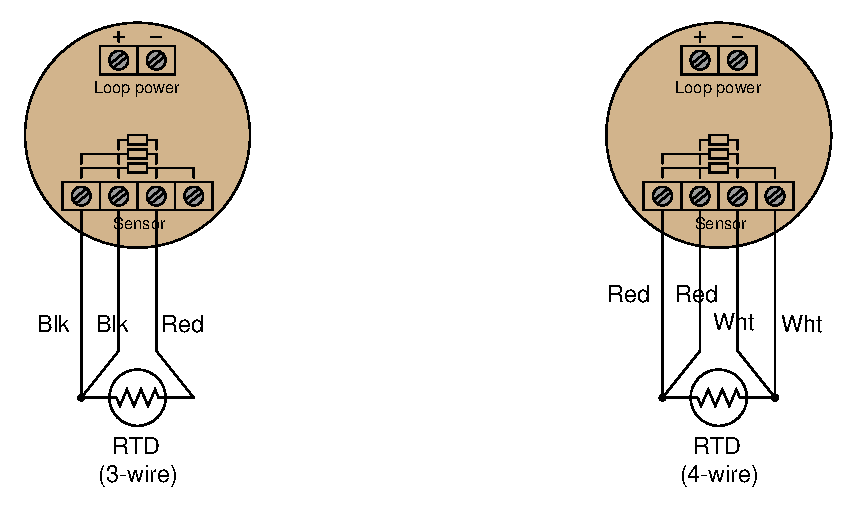
\includegraphics[width=15.5cm]{i00404x03.eps}$$

%(END_ANSWER)





%(BEGIN_NOTES)


%INDEX% Measurement, temperature: RTD

%(END_NOTES)
